\begin{center}
\Large \textbf{Chapter 2: Theories of Lexical Decomposition} \\[1ex]
\end{center} 
 \setcounter{section}{0}
In this chapter, we will identify two properties that are shared by all decompositional theories, one essential and one (seemingly) accidental. It is essential to a theory of lexical decomposition that it includes some sort of semantic \emph{atom} in its ontology; decomposition simply \emph{is} breaking semantic content down into atoms. Although not essential to decomposition per se, we will observe that the atoms of all decompositional theories are related to each other by \emph{inheritance}. Inheritance is a reflexive and transitive relation in which information is said to be \emph{inherited} by one atom from another. If an atom $\alpha$ inherits from an atom $\beta$, information obtained about $\beta$ will generally apply to $\alpha$. The interpretation of atoms offered in this thesis will explain why inheritance appears in decomposition so consistently, turning this accidental property into an essential one.

To begin, we will look at some examples of lexical decomposition, highlighting those aspects of each theory that are relevant to the present discussion. Each theory is formulated within its own framework, based on whatever set of foundational assumptions are held by each theorist: Jackendoff models internal representations of meaning, as a total theory of semantics, while Levin and Rappaport Hovav model the semantic features of verbs that have consequences for syntax. James Pustejovsky's \emph{Generative Lexicon} (GL) seeks to improve on traditional lexicons by decomposing words in a way that allows new word senses to be generated, rather than requiring all word senses to be stored in the lexicon as independent entries. We will not here be concerned with these foundational differences; regardless of which approach to lexical decomposition we look at, the general \emph{method} of analysis---the method of composing meaning out of atoms, by means of some structural rules of composition---is the same. Our primary concern here is to understand this general method, rather than the nitty-gritty details of each individual theory.

\section{Formal Theories of Lexical Decomposition}\label{sec2.1}

\subsection{Jackendoff's cognitive semantics}

The meaning of a lexical item (or a portion of its meaning, at least) is given in a \emph{feature structure} in which types are assigned to different ``features'' or aspects of the word's meaning. The basic form of one of Jackendoff's feature structures is:
\par\vspace{5mm}
$\left[
\begin{array}{l}
\textbf{event, thing, place,}\mathellipsis \\
\text{token/type} \\
F(\langle\text{Entity}_1,\langle\text{Entity}_2,\langle\text{Entity}_3\rangle\rangle\rangle)
\end{array}
\right]$
\par\vspace{5mm}
The top feature in the structure specifies an \emph{ontological category} under which the lexical item falls. Ontological categories provide a partition of the ways in which our cognitive architecture allows us to represent word meaning. The middle feature is an immediate \emph{inheritance relation} (explained below) in which the word participates (normally by specifying a type from which the word's meaning inherits),\marginpar{This is where I have addressed your question about how to interpret {\bf book} in the feature structure for {\bf novel}. I modified the wording very slightly to make it more consonant with the way you put the point, because what you said is what I think is right.} and the third and final feature is the argument\footnote{Jackendoff uses the term ``argument'' here in a non-linguistic sense, i.e.\ it does not mean ``grammatical argument.'' He does little to explain what other sense of ``argument'' he is using, but since everything he calls an argument is an input to the function $F$, I read him as using ``argument'' in the sense of arguments of a function. $F$ is a \emph{cognitive mapping} from properties onto meanings, i.e.\ concepts, which is inherent in biology of human cognition. In the case of verbs, the functional arguments turn out to be the grammatical arguments.} structure of the word, i.e.\ the types of arguments that the word can take, which will change depending on the sense in which the word is being used. For example, take the following typed feature strucutures for ``novel'' and ``begin'':
\par\vspace{5mm}
{\bf novel}
$\left[
\begin{array}{l}
\textbf{thing} \\
\textbf{book} \\
F(\langle\textbf{property}\rangle)
\end{array}
\right]$
\par\vspace{5mm}
{\bf begin}
$\left[
\begin{array}{l}
\textbf{event} \\
\textbf{transition} \\
F(\langle\textbf{animate\_object},\langle\textbf{event}\rangle\rangle)
\end{array}
\right]$
\par\vspace{5mm}

``Begin'' takes a primary argument of type {\bf animate\_object} (since only animate objects can begin actions) and a secondary argument of type {\bf event} (since only events can be begun).\footnote{We might quibble over whether these type assignments are the \emph{right} ones for ``begin.'' It's not important here whether I accurately convey the specific types involved in the semantics of ``begin,'' and these will suffice at least to get a handle on how Jackendoff's feature structures are supposed to work, which is the real goal here.} ``Novel'' might take arguments of type {\bf property}, as it is used in the sentence ``This novel is long''; but, in the sentence ``The novel is on the table,'' the argument type is {\bf place}. These are differences between senses of ``novel,'' which are largely determined by the syntactic structure of the sentence and a grammatical conceptual structure inherent in human cognition. The details of how this works are interesting, but not relevant to the present project.

The ontological category and immediate inheritance relation, however, \emph{are} relevant to the present project, so it is useful at this point to explain them.

Jackendoff's types are organized according to the \emph{inheritance relation} $\sqsubseteq$.\footnote{Jackendoff does not call the relation inheritance; I have modified his terminology in order to make my own terminology consistent throughout this paper. He calls the relation an ``IS-A'' relation or a ``type-token'' relation, both of which are fairly common alternatives.} Inheritance is reflexive and transitive, but not symmetric. Given two atoms $\alpha$ and $\beta$ such that $\alpha\sqsubseteq\beta$, we say that $\alpha$ inherits from $\beta$. Or, $\alpha$ is a \emph{subtype} of $\beta$. If there is a third atom $\gamma$ such that $\beta\sqsubseteq\gamma$, then what the inheritance relation tells us is that $\alpha\sqsubseteq\gamma$ as well. If we let {\bf x} be a member of any domain to which the types can apply, we write {\bf x}:$\alpha$ to indicate that {\bf x} is of type $\alpha$. By inheritance, {\bf x}:$\alpha\vdash${\bf x}:$\beta\vdash${\bf x}:$\gamma$.

The broadest type, of which all other types are subtypes is the type {\bf entity}. Beneath {\bf entity}, there is a set of \emph{ontological categories}, none of which inherit from each other, but all of which inherit from {\bf entity}. These are {\bf thing}, {\bf event}, {\bf state}, {\bf action}, {\bf place}, {\bf path}, {\bf property}, and {\bf amount}. This sort of system might remind the reader of Aristotle's \emph{Categories}, which might be regarded as the earliest example of a type-inheritance theory of lexical semantics. Every lexical item will fall under one of the ontological categories.

At first glance, Ray Jackendoff seems to advocate a version of my own view. In \cite{jackendoff_semantics_1983}, he argues that word meaning is decomposed into concepts, but his usage of the word ``concept'' is broader than mine. For Jackendoff, a concept is any mental representation, and it includes subjective representations of categories (which is, more or less, what cognitive scientists mean when they talk about concepts), subjective representations of propositions, mental representations of individual objects, and perhaps even the cognitive structural rules which Jackendoff believes to be the source of basic grammatical structure for natural languages.

Jackendoff's notion of concept is too broad to do the work that will be required here. The connection I draw between semantic and conceptual content will rely on empirical results pertaining to the hierarchical organization of concepts (in the cognitive scientist's sense). These results have not been seen for other mental representations.

Moreover, his notion of concept is entirely subjective; that is, Jackendoff's concepts explicitly have no important connection to the external world. This is largely due to his view on the nature of mind, which is little more than a more readable rendition of Kant's \emph{Transcendental Aesthetic} \cite[Ch. 2]{jackendoff_semantics_1983}. Our faculty of sensation is somehow roused into action by external stimuli. Sensations are used as a kind of paint by the mind, which creates a subjective picture or ``projected world'' (cf.\ Kant's phenomenal world) by applying the paint in accordance with concepts, which act as a kind of blueprint. It is concepts, not the external world, that determines what we see in the projected world. And the projected world is \emph{all} we see, all our words can possibly refer to. One of our goals here is to explain how words hook up with the external world, but Jackendoff (and Kant) have reinterpreted the word ``world'' in such a way that it becomes non-sensical to talk about the external world at all.

I have serious reservations about whether Jackendoff should be allowed to reinterpet ``world'' in this way, but arguing this point belongs to an entirely different project. For the present purpose, it is taken as an explicit assumption that our words do connect with the external world in some way. Under this assumption, we then ask the question ``How do words connect to the external world?'' Since Jackendoff has explicitly denied that words (or concepts) have any important relation to the external world, making this assumption places us outside the scope of Jackendoff's framework.

Nevertheless, Jackendoff's theory is decompositional and therefore exhibits the same features of other decompositional theories that will be important here. Where decomposition is concerned, it is type ``concepts'' (in the Jackendoff-ian sense) that are taken as atomic.  

As will be seen below, there will be a fundamental connection between these parts of the feature structure and semantic content. Before spelling out this connection explicitly, however, we will look at a few more examples of lexical decomposition.

\subsection{Levin and Rappaport Hovav's verb decomposition}

In \cite{levin_building_1998}, Levin and Rappaport Hovav offer a decompositional semantics for verbs specifically. In particular, they model those aspects of verb semantics that have consequences for which grammatical arguments must be, might be, or cannot be syntactically realized in a sentence. Like Jackendoff, they hold the view that there is some definite set of ontological categories that can be invoked as part of the semantic theory, i.e.\ there is some universal set of atoms from which all verb meaning is constructed. In fact, they accept Jackendoff's ontological categories, \emph{plus} an additional set of fixed ontological categories that inherit from Jackendoff's {\bf event} type. Among these additional ontological categories are {\bf cause}, {\bf become}, and {\bf act}; in another paper \cite{levin_lexical_2008}, they give a long list of others that are commonly seen in theories of verb decomposition. The subtypes of Jackendoff's other ontological categories (which are not dubbed as ``ontological categories''), are left explicitly open-ended; that is, they can be whatever and however many in number are required to give a semantic analysis of all verbs in a natural language.

Some of the ontological categories in this additional set are called \emph{predicates}, and they will determine the structure of the semantic entry (while arguably simultaneously providing some semantic content), while the others are called \emph{constants}, which only provide semantic content and act as arguments for the predicates.

We cannot give a semantic entry for ``novel'' in their system, since it deals only with verbs, but we can give an entry for ``begin'':
$$[[ x\textbf{ act}]\textbf{cause}[x\langle\textit{ACTION}\rangle]],$$
where \emph{ACTION} is a variable standing for any subtype of the constant {\bf action}. If some agent $x$ \emph{begins} to perform some \emph{action}, then $x$ \emph{acts} to \emph{cause} $x$ to be in a state of \emph{action}. For example, the event structure for the event described by (2) ``Maria began reading'' is
$$[[ \text{Maria}\textbf{ act}]\textbf{cause}[\text{Maria} \langle\textbf{reading}\rangle]].$$

Again, we have a set of atoms that provide semantic content, i.e.\ the constants. And again the use of these atoms relies on an inheritance relation: inheritance from {\bf action} is a constraint placed on the content of arguments for ``begin.''\footnote{Section 3.1 of this chapter includes some more examples of this kind of constraint. All three examples in this section are in the Levin class of \emph{change of state} verbs, which share the structural template $[\textbf{become}[y\langle\textit{RES-STATE}\rangle]]$. Any constant that can serve as a value for the variable \emph{RES-STATE} must be a subtype of the constant {\bf resulting\_state}.}

Levin and Rappaport Hovav's semantic theory is not merely an abstract exercise. Computational lexical resources exist which have real-world technological implementations such as automated translation, corpus annotation, treebanking, automated sentence parsing. These implementations are useful for application in artificial intelligence, speech recognition, language learning software, etc.

VerbNet, a lexical resource created and managed by Karin Kipper-Schuler, Martha Palmer, and others at University of Colorado, is currently the largest on-line verb lexicon for English. Lexical entries are organized into verb classes based on the predicates of Levin and Rappaport Havov\footnote{In VerbNet, the predicates are called \emph{thematic roles}, following \cite{Jackendoff_semantic_1972}, but they come down to the same thing as Levin and Rappaport Havov's predicates. I call them predicates because I have already introduced this term and VerbNet is explicitly based on their theory.}, and it is perhaps in the implementation that we can most-readily observe the type-inheritance system of Levin and Rappaport Hovav's content-bearing constants (or atoms).
\par\vspace{3mm}
\begin{figure}[h]
  \centering
      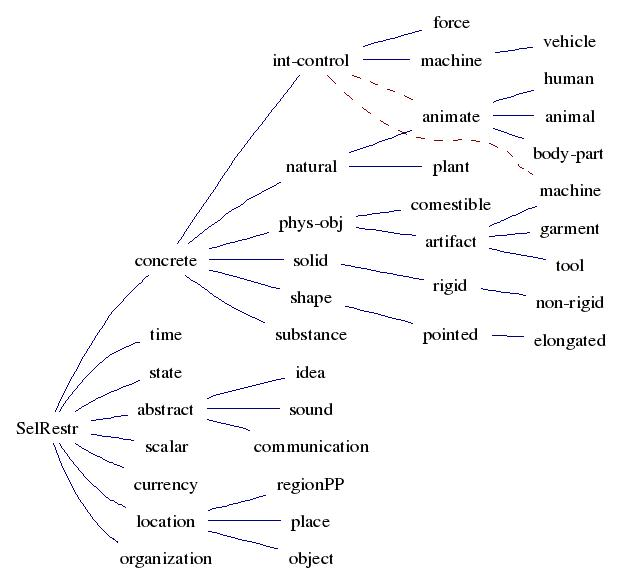
\includegraphics[width=4in]{./Chapters/Ch2/verbnetinheritance.jpg}
  \caption{A sample type inheritance hierarchy from VerbNet}
\end{figure}

\section{Moral of the story: Lexical Semantic Content and Inheritance}

\subsection{Lexical Semantic Content}

In any decompositional theory, there is a structural component and a content-providing component. Levin and Rappaport Havov \cite{levin_lexical_2008} have made this exact point for their own theory (and others in the same general subclass of theories of lexical decomposition). Although their theory is a theory of verb decomposition, their comments apply to lexical decomposition in general. Many words might have the same general structure for Levin and Rappaport Hovav's lexical entries, only differing in their semantic content, which is represented in the form of semantic atoms. For example, given the structural template $[\textbf{become}[y\langle\textit{RES-STATE}\rangle]]$, where \emph{RES-STATE} is a variable ranging over the domain of resulting states, we have the following three lexical entries:\footnote{``Lexical entry'' is a general term that applies to any structure or item that is used to convey the meaning of a word in the lexicon of a semantic theory.}
\begin{enumerate}
\item \emph{dry}: $[\textbf{become}[y\langle\textbf{dry}\rangle]]$
\item \emph{widen}: $[\textbf{become}[y\langle\textbf{wide}\rangle]]$
\item \emph {dim}: $[\textbf{become}[y\langle\textbf{dim}\rangle]]$
\end{enumerate}
It is obvious that ``dry,'' ``widen,'' and ``dim'' all have very different meanings, yet the structure of these lexical entries is the same, different only in the atom that occurs in the argument for {\bf become}. The part of each lexical entry that is idiosyncratic to each word is the content provided by the atom. The same point applies to Jackendoff, and, as we'll see below, to the Generative Lexicon theory \cite{pustejovsky_generative_1998}.

In lexical decomposition, semantic content is always inherited from some basic atom. But this is only possible if atoms have content, so it makes sense to inquire after the content of atoms. 

David Lewis \cite{lewis_general_1970} has given a compelling argument in the domain of sentential decomposition that atoms must be given an interpretation in order for a semantic theory to do any of the work we require from such a theory. A decompositional theory provides a set of atoms or ``markers,'' which are essentially a lexicon for the theory. The compositional rules provide a syntax according to which we combine the atoms into some sort of structure representing the semantics of whatever linguistic unit is in the domain of the theory (in Lewis's case, the linguistic units under consideration are sentences; in ours, they are words). ``But,'' Lewis writes,
\begin{quote}
we can know the Markerese translation of an English sentence without knowing the first thing about the meaning of the English sentence: namely, the conditions under which it would be true. Semantics with no treatment of truth conditions is not semantics. Translation into Markerese is at best a substitute for real semantics, relying either on our tacit competence (at some future date) as speakers of Markerese or on our ability to do real semantics at least for the one language Markerese.
\end{quote}
Proponents of decompositional theories are able to get by without providing content to their atoms precisely because they and their audience are speakers of the relevant ``Markerese.'' In all theories considered here, the atoms are represented in English. Since we are all able to understand the words represented by these signs, in virtue of the fact that we are all fluent speakers of that natural language, we are able to make sense of decompositional lexical entries even without a ``real semantics'' for English or Markerese. Theorists of lexical decomposition rely on fluency to supply content to atoms where none is given within the theory. One of the main goals of this project is precisely to indicate one way in which we can do ``real semantics'' for Markerese, at the same time situating our decompositional theories within the broader context of ``real semantics'' for natural language.

If we follow Lewis in thinking that uninterpreted atoms do not have content, but want to retain the decompositional approach, then we will want to compose word meaning out of some atom whose content we understand independently of the decompositional theory. Absent some interpretation that provides content to atoms from without, it is difficult to see how we might obtain such understanding. Any theory of lexical decomposition is necessarily unable to non-circularly provide content to its atoms. Within the theory, the meanings of atoms can only be decomposed into other atoms; theories of lexical decomposition are \emph{only} theories of lexical decomposition. But if the meanings of atoms are given decompositionally, then either: (a) they aren't \emph{actually} atoms of the theory; (b) we will ultimately bottom out with the meanings of some atoms given in terms of themselves; or (c) we have a ``decompositional circle,'' e.g.\ $\alpha$ is defined in terms of $\beta$ and $\gamma$, $\beta$ is defined in terms of $\delta$ and $\phi$, and so on, until we reach some atom defined in terms of $\alpha$. In any case, we cannot form a coherent view of how a decompositional theory can provide meaning to its own atoms. The current external source of content for atoms is their identification with English words, which retrieve content from fluency of native speakers. But if this is the actual source of content for the atoms, then we have an obvious circularity: linguistic items supply content to atoms, which supply content to linguistic items.

Nevertheless, linguists and philosophers alike (many of them at least) seem to agree that decompositional theories play a crucial role in semantics as a whole.\footnote{In the domain of sentential semantics, it is wholly uncontroversial that decomposition is the right approach. There is some controversy over lexical decomposition, and die-hard opponents of lexical decomposition may reject what is said here. Justifying lexical decomposition is outside the scope of this paper; I seek to fortify lexical decomposition, given that we already agree on the appropriateness of the decompositional approach to word meaning.} It is not the case that lexical decompositional theories are completely useless until and unless we can find ourselves in possession of a convincing account of the content of its atoms. Any lexical decompositional theory comprises only part of a total science of lexical semantics. Decompositional theories can tell us a great deal about the structural component of meaning.

However, we take ourselves to be talking \emph{about} something when we use words, and except when what we are actually talking about is atoms, to say that atoms are the providers of the content component of meaning doesn't tell us what our words are \emph{about}. When I say, ``The sky is clear today,'' I've said nothing at all about atoms. I've said something about the sky. Whatever sort of thing meaning is, \emph{aboutness} is a major component of it. We might say that ``The sky is clear today'' is about the sky because the word ``sky'' refers to the sky. This is on the right track, but some words have meaning without referring to anything, e.g.\ unicorn, goblin, etc., so reference cannot be a necessary condition of meaning. As a guiding intuition, we might say: When a word has reference, its reference plays an important role in meaning. In cases where a word has no reference, some story will need to be told about the meanings of words, but I think that what I will argue is compatible with any plausible story that might be offered.

My proposal is that we can identify some cognitive representation---namely, concepts---that is generally agreed to be \emph{about} something, and which will hook up with the world in some way in cases where references exist in the world. If we are able to do this, we will be able to satisfy referentialists such as Lewis, by allowing our cognitive structures to mediate between words and reference while also being palatable to subjectivists such as Jackendoff, who wish to give a theory of internal semantics in which linguistic units have no direct reference beyond what is present in the mind.

We have now identified in passing a number of criteria that will justify concepts as an appropriate interpretation of semantic atoms. It will serve us well to review them explicitly. Two problems with the current situation have been mentioned: there is no coherent, non-circular way for decompositional theories to provide content to their own atoms without relying on prior understanding of the meanings of words; without content for the atoms, we are unable to account for \emph{aboutness}. Also, we should keep in mind that atoms are supposed to be carriers of semantic content; therefore, any viable interpretation must exhibit some behavior that reflects fundamental observations about semantic content. At this point, we are able to identify three criteria that a successful interpretation of the atoms must meet. I will take the current project to have been successful when I have established an interpretation that
\begin{enumerate}[(i)]
\item accounts for \emph{aboutness},
\item is not itself dependent on linguistic meaning, and
\item explains why inheritance networks appear in all theories of lexical decomposition, despite the fact that inheritance is not essential to decomposition \emph{per se}.
\end{enumerate}

\section{James Pustejovsky's Generative Lexicon}\label{GL}

James Pustejovsky's theory of lexical decomposition, the Generative Lexicon (GL) \cite{pustejovsky_generative_1998} will provide a case study for developing the conceptual interpretation of semantic atoms, so it will be useful to look at GL in some level of detail.

GL is a theory of lexical semantics based on LKB \cite{sanfillipo_lkb_1993}, which is in turn based on Bob Carpenter's logic of typed feature structures \cite{carpenter_logic_1992}. GL is a model of word meaning in which the mechanisms underlying systematic polysemy allow new word senses to be generated ``on the fly,'' without their being given explicitly in the lexicon. Historically, the simplest and most direct means of handling polysemy has been to allow the same word to be listed multiple times in the lexicon, with each listing storing a different semantics for the word. A precise characterization of this sort of \emph{Sense Enumeration Lexicon} SEL is
\begin{quote}
A lexicon $L$ is a \emph{Sense Enumeration Lexicon} if and only if for every word $w$ in $L$, having multiplie senses $s_1,\mathellipsis,s_n$ associated with that word, then the lexical entries expressing these senses are stored as $\{w_{s_1},\mathellipsis,w_{s_n}\}$. \cite[p. 34]{pustejovsky_generative_1998}
\end{quote}

The inadequacies of SELs are spelled out detail by Pustejoveky \cite[Ch.\ 4]{pustejovsky_generative_1998}, and for a fuller discussion of them, the reader is referred to his book. They are not important for our purposes here. What is important is that Pustejovsky capitalizes on the well-known phenomenon of systematic polysemy as a way of reducing the number of entries in the lexicon. To understand what systematic polysemy is, it is helpful to distinguish it from polysemy (simpliciter) and lexical abiguity (or homophony). Polysemy (simpliciter) is the capacity that some words possess to take on multiple distinct, but related meanings. For example, we use the word ``dog'' to refer to both actual dogs, drawings of dogs, or even humans whom we call dogs pejoratively to indicate unsavory behavior. However, not all cases of using a common morpheme to refer to different things are cases of polysemy. The very common example of ``bank,'' which can refer to a financial institution or the land beside a river, is not an example of polysemy, but of lexical ambituity (or homophony). These meanings are entirely unrelated, and in fact it is common for linguists to regard these uses of ``bank'' as entirely different words, which share a phoneme through historical accident. A \emph{systematic polysemy} arises when it is achieved in accordance with some regular, generally established \emph{generative rule} according to which word senses can be produced in a predictable way.

\subsection{Typed Feature Structures}

In the GL, the semantics of a lexical item $\alpha$ is represented as a quadruple $\langle \mathcal{A},\mathcal{E},\mathcal{Q},\mathcal{I}\rangle$. Each component is discussed below. The inheritance structure $\mathcal{I}$ is covered first, since it is the main one we are concerned with here. $\mathcal{A}$ and $\mathcal{Q}$ will become useful in Chapter 5. $\mathcal{E}$ is included for completenes, but it is not essential to understanding what follows.

\subsubsection{The lexical inheritance structure $\mathcal{I}$.}

The lexical inheritance structure $\mathcal{I}$ is a lattice which defines what is to be considered as a type for atoms and the relations between types. Following Carpenter's Logic of Type Feature Structures, the fundamental relation between types is inheritance. The inheritance lattice is a partial ordering $\sqsubseteq$ over types and we say that $\alpha$ \emph{inherits from} $\beta$ just in case $\alpha\sqsubseteq\beta$. If $\alpha$ inherits from $\beta$, then $\alpha$ is a \emph{subtype} of $\beta$, i.e.\ for any object {\bf x}:$\alpha$, it is also the case that {\bf x}:$\beta$. The entire logic of typed feature structures is a spelling-out of the consequences of the inheritance relation. We do not need to be too concerned with the details of the logic here and can simply refer to Carpenter's work where necessary. A sample inheritance lattice is given below:
\par\vspace{5mm}
\xymatrix{
& \textbf{phys\_obj} & & \textbf{information} \\
\textbf{organization} & & \textbf{print-matter} \ar@{->}[ul] \ar@{->}[ur] & \\
& \textbf{newspaper} \ar@{->}[ul] \ar@{->}[ur] & \textbf{book} \ar@{->}[u] & \textbf{narrative} \ar@{->}[uu] \\
& & & \textbf{novel} \ar@{->}[ul] \ar@{->}[u] }
\par\vspace{3mm}
\begin{center}Figure 2\end{center}
\par\vspace{3mm}

Neither Pustejovsky nor Carpenter commits us to any specific inheritance structure, nor even a specific set of types. Carpenter, in particular, is explicit that, so far as his logic is concerned, any set of types and any inheritance structure will do, provided they possess a certain set of very general characteristics. We need not be too concerned with Carpenter's conditions; it will be difficult to cook up any set of types or inheritance relations which do not meet them, but which are also plausible for use in the GL. A more important issue arises from the fact that Pustejovsky does not consider the question of whether there are some inheritance structures that are better than others for modeling word meaning. Indeed, Pustejovsky doesn't say much about $\mathcal{I}$ at all, other than what it is. In Chapter 4, a proof will be given that there is an important relation between the hierarchical organization of concepts and inheritance structures and that, by giving an appropriate model of concepts which is sufficient to explain hierarchy, we can get greater insight into $\mathcal{I}$. Importantly, it is my hope that we will get some answer to the question of whether any $\mathcal{I}$ at all will do, or whether only some $\mathcal{I}$s are viable candidates as part of a linguistic structure in the GL.

\subsubsection{The argument structure $\mathcal{A}$.}

Argument\footnote{Like Jackendoff, Pustejovsky's use of the term ``argument'' is somehwat misleading for linguists. Pustejovsky's arguments are also arguments of some function. His formal system is explicitly based on Ann Copestake's LKB \cite{copestake_implementing_2002}, whose argument structures are explained as inputs to computational functions defined when a grammar is implemented in LKB.} structure is the best-understood of the components and is regarded as a minimal specification of lexical semantics, although it is far from adequate as a complete characterization of the semantics of any lexical item.

The grammatical arguments of the lexical item ``build'' are encoded into a list structure ARGSTR in the following manner:
\par\vspace{5mm}
$\left[
\begin{array}{l l}
\textbf{build} & \\
\text{ARGSTR} = & \left[ \begin{array}{l}
				\text{ARG}_1=\textbf{animate\_individual} \\
				\text{ARG}_2=\textbf{artifact} \\
				\text{ARG}_3=\textbf{material}
				\end{array}\right] \\
\mathellipsis &
\end{array}
\right]$
\par\vspace{5mm}
\noindent For a verb, the argument structure will give an account of the grammatical arguments expected by the verb, while for a non-verb, the argument structure will correspond, roughly, to the word's behavior when used as the argument for a verb. Arguments corresponding to the subject are indexed with 1, direct objects with 2, indirect objects with 3, 4, 5, etc. This is best understood through example; Chapter 5 will provide a number of examples that illustrate the argument behavior of non-verbs.

\subsubsection{The extended event structure $\mathcal{E}$.}

The extended event structure will not be important for the purposes of this thesis and is included merely for completeness and to prevent the reader from feeling overwhelmed by their presence in the typed feature structures that will be used in Chapter 5. The following is an example of the event structure for the word ``build'':
\par\vspace{5mm}
$\left[
\begin{array}{l l}
\textbf{build} & \\
\text{EVENTSTR} = & \left[ \begin{array}{l}
				\text{E}_1=\textbf{process} \\
				\text{E}_2=\textbf{state} \\
				\text{RESTR}=<_\alpha
				\end{array}\right] \\
\mathellipsis &
\end{array}
\right]$
\par\vspace{5mm}
\noindent The $\text{E}_i$ are features that correspond to the stages of an event that extends through time. In the above example, the act of building something involves a \emph{process} (of building), and it ends with an object being in a \emph{state} of having been built. The feature RESTR defines the order that is placed over stages of an event, e.g.\ total ordering, partial ording with simultaneity, partial ordering without simultaneity. $<_\alpha$ is Pustejovsky's symbol for a total order (without simultaneity), which is perfected or completed with the final stage of the event; building ends when the thing we are building is in a state of having been built, and the act of building and the state of having been built cannot occur simultaneously.

\subsubsection{The qualia structure $\mathcal{Q}$.}

Pustejovsky's qualia structure is borrowed from Aristotle's four modes of explanation or four causes. The analysis given here will not depend on a detailed understanding of what the qualia are; we need only understand that they provide semantic information that should be accessible by native speakers of a language when they use a word.  In fact, generative lexicons can be created in which the generative mechanisms depend on features other than qualia structure, so there is nothing essential about Pustejovsky's choice of qualia. His choice of the qualia is largely predicated on Moravcsik \cite{moravcsik_aitia_1975}, who argues that Aristotle's four causes serve as a generative mechanism for creating new word senses.  The qualia structure QUALIA is constituted by assigning types to the four following features:
\begin{enumerate}
\item \emph{Constitutive.} The material properties of an object; the relation between an object and its  proper parts. Some examples are:
	\begin{enumerate}
	\item Material
	\item Weight
	\item Parts and component elements
	\end{enumerate}
\item \emph{Formal.} The property according to which an object of a particular species is regarded also as a member of some broader genus. Some examples are:
	\begin{enumerate}
	\item Orientation
	\item Magnitude
	\item Shape
	\item Dimensionality
	\item Color
	\item Position
	\end{enumerate}
\item \emph{Telic.} The purpose or function of an object. Some examples are:
	\begin{enumerate}
	\item Purpose for which an object was created by some agent.
	\item A built-in function or aim toward which the natural activities of an object point.
	\end{enumerate}
\item \emph{Agentive.} The origin of an object or factors involved in its ``bringing about.'' Some examples are:
	\begin{enumerate}
	\item Creator
	\item Artifact
	\item Natural kind\footnote{Pustejovsky lists this, but I am hesitant to do the same, due to some confusions and/or skepticism I have pertaining to natural kinds, which are off-topic from the present discussion.}
	\item Causal Chain
	\end{enumerate}
\end{enumerate}

As an example, consider the following QUALIA structure for ``novel'':
\par\vspace{5mm}
$\left[
\begin{array}{l l}
\textbf{novel} & \\
\mathellipsis & \\
\text{QUALIA} = & \left[ \begin{array}{l}
				\text{CONST}=\textbf{narrative} \\
				\text{FORMAL}=\textbf{book} \\
				\text{TELIC}=\textbf{reading} \\
				\text{AGENT}=\textbf{writing}
				\end{array}\right] \\
\end{array}
\right]$
\par\vspace{5mm}
This simple listing of qualia values ``tells us nothing about how a particular lexical item denotes, however. For example, although a novel's purpose is the activity of reading and it comes about by someone writing it, we do not want to claim that the common noun \emph{novel} actually denotes such activities'' \cite[pg.\ 78]{pustejovsky_generative_1998}. The qualia provide information \emph{about} what is denoted by the word.

\clearpage
